\documentclass[a4paper]{article}

%\usepackage{fullpage}
\usepackage[14pt]{extsizes}			% размер шрифта
\usepackage[T2A]{fontenc}			% кодировка
\usepackage[utf8]{inputenc}			% кодировка исходного текста
\usepackage[english,russian]{babel}	% локализация и переносы
\usepackage{mathtools}				% математический пакет (включает ams)
\usepackage{amssymb}				% для \leqslant
\usepackage[thinc]{esdiff}			% производные
\usepackage{graphicx}				% изображения
\usepackage{wrapfig}				% Обтекание рисунков и таблиц текстом
\usepackage{listings}				% програмный код
\lstset{
	numbers=left               
}
\usepackage{setspace}
\onehalfspacing						% полуторный интервал

%\usepackage{afterpage}				% geometry для индивидуальной страницы
\usepackage{geometry}

\usepackage{tocloft}				% точки в содержании для \section
\usepackage{cleveref}				% несколько ссылок \cref
\renewcommand{\cftsecleader}{\cftdotfill{\cftdotsep}}
\usepackage{siunitx}				% единицы СИ 
									%Number only: \num{1e-10}
									%Number with units: \SI{1e-10}{\meter\per\second}
\author{Бартая Нодари ФМ-101}
\title{ОТЧЁТ\\ Отчёт о НИР}
\date{\today}

\begin{document}

\begin{titlepage}
	\begin{center}
		Федеральное государственное бюджетное образовательноe учреждение высшего образования \\
		\textbf{«Челябинский государственный университет» \\ (ФГБОУ ВО «ЧелГУ»)}
	\end{center}
	\begin{center}
		Факультет физический			\\
		Кафедра теоретической физики	\\
		Направление 03.04.02 Физика		\\
		Направленность Теоретическая и математическая физика
	\end{center}
	\vfill
	\begin{center}
		\textsc{\textbf{Отчёт о научно-исследовательской работе}}
	\end{center}
	\vfill
	\singlespace
	\begin{flushright}
		\begin{tabular}{r p{0.4\textwidth}l}
			Преподаватель:&	доцент кафедры теор. физики, кандидат физ.-мат.наук 
			
			Хайбрахманов С.А. \\[5pt]
			Студент:&	Бартая Н.В.		\\[5pt]
			Группа:& 	ФМ-101			\\
		\end{tabular}
	\end{flushright}
	\onehalfspacing
	\vfill
	\begin{center}
		Челябинск, 2020	
	\end{center}
\end{titlepage}

\begin{titlepage}
	\newgeometry{margin=2cm, footskip=0pt, hoffset=-5pt}
	\singlespacing
	\begin{center}
		Федеральное государственное бюджетное образовательноe учреждение высшего образования \\
		\textbf{«Челябинский государственный университет» \\ (ФГБОУ ВО «ЧелГУ»)}
	\end{center}
	\begin{center}
		Факультет физический			\\
		Кафедра теоретической физики	\\
		Направление 03.04.02 Физика		\\
		Направленность Теоретическая и математическая физика
	\end{center}
	\vfill
	\begin{center}
		\textbf{ИНДИВИДУАЛЬНОЕ ЗАДАНИЕ\\на научно-исследовательскую работу}
	\end{center}
	%\singlespace
	\begin{center}
		\begin{tabular}{p{0.35\textwidth} p{0.68\textwidth}}
			Студент					&	Бартая Нодари Вахтангович	\\
			Академическая группа	&	ФМ-101						\\
			Место прохождения \hfill \newline
			практики:	&	ФГБОУ ВО «ЧелГУ», кафедра теоретической физики						\\
			Срок прохождения \newline практики: & 30 – 31 декабря 2019 г. и 9 – 20 января 2020 г.
		\end{tabular}
	\end{center}
\vfill
\raggedright Перечень заданий и вопросов, подлежащих исследованию:
\begin{enumerate}
	\item Изучить двухшаговый метод Лакса-Вендроффа.
	\item Реализовать метод в виде кода на языке С\textbackslash С++.
	\item Протестировать код на задаче о линейном переносе и на задаче о распаде произвольного газодинамиечкого разрыва.
\end{enumerate}
	\vfill
	\onehalfspacing
	Руководитель от профильной организации \enspace\hrulefill \hspace{0.2cm} С. А. Хайбрахманов,
	
	доцент кафедры теоретической физики, кандидат физ.-мат. наук \vspace{3pt}
	
	Руководитель от образовательной организации \enspace\hrulefill \hspace{0.2cm} А.Е. Дудоров,
	
	зав. кафедрой, доктор физ.-мат. наук, профессор \vspace{3pt}
	
	Задание к исполнению принял \enspace\hrulefill \hspace{0.2cm} Н.В. Бартая
	
	
	\vfill
	\begin{center}
		Челябинск, 2020	
	\end{center}
\end{titlepage}
\restoregeometry	

\tableofcontents
\setcounter{page}{3}
\newpage

	\section*{Введение}
	В отчёте представлено решение поставленных в индивидуальном задании задач. Исследуются решения уравнений сплошной среды. Численный метод рассмотрен в разделе \ref{Lax-Wendroff}. 
	Задача о линейном переносе и о произвольном гидродинамическом разрыве описаны в разделах \ref{transfer} и \ref{hydrodynamics}, соответственно.
	
	\section{Двухшаговый метод Лакса-Вендроффа}\label{Lax-Wendroff}
	Разностые методы применяются для расчёта различных физических задач с использованием вычислительной техники. В этой работе будет исследоваться применение двухшагового метода Лакса"=Вендроффа, для уравнений вида: 
	\begin{equation}\label{dudt}
	\diffp{\mathbf{u}}{t} + \diffp{\mathbf{F}}{x} = 0 ,
	\end{equation}
	где $\mathbf{u}$ называют вектором консервативных переменных, $\mathbf{F}$ - вектором потоков соответствующих физических величин.
	
	Уравнение \ref{dudt} является уравнением гиперболического типа. Интегрирование будет проводиться с помощью явного, консервативного метода второго порядка точности как по пространству, так и по времени. Непрерывные производные аппроксимируются конечными разностями, далее вычисление проходит в два этапа - предиктор, корректор. 
	
	Первый этап также называют вспомогательным шагом, он производится на каждом шаге по времени и позволяет получить значения величин и их потоков в промежуточные моменты времени, тем самым центрируя по времени интеграл и позволяя получить точность второго порядка \cite{Potter}. Схема метода представлена на рисунке \ref{LW_picture}.
		
	\textit{Вспомогательный шаг:}
	\begin{equation}\label{LW_helper}
	\mathbf{u}_{j+1/2}^{n+1/2} = \frac{1}{2} \left(\mathbf{u}_{j}^{n} + \mathbf{u}_{j+1}^{n}\right)
	- \frac{\Delta t}{2 \Delta x}
	\left(\mathbf{F}_{j+1}^{n} - \mathbf{F}_{j}^{n}\right) .
	\end{equation}
	Далее, полученные значения используются для нахождения потоков в промежуточных временных и пространственных точках:
	\begin{equation}\label{LW_flow}
	\mathbf{F}_{j+1/2}^{n+1/2} = \mathbf{F} \left( \mathbf{u}_{j+1/2}^{n+1/2} \right).
	\end{equation}
	На втором этапе, используя промежуточные величины, вычисляется новый временной слой.
	
	\textit{Основной шаг:}
	\begin{equation}\label{LW_main}
	\mathbf{u}_{j}^{n+1} = \mathbf{u}_{j}^{n} - \frac{\Delta t}{\Delta x} \left(
	\mathbf{F}_{j+1/2}^{n+1/2} - \mathbf{F}_{j-1/2}^{n+1/2}				 \right) .
	\end{equation}
	Условием устойчивости метода является так называемое число Куранта $C \leqslant 1$, что равносильно условию Куранта -- Фридрихса -- Леви, применимого ко всем уравнением гиперболического типа: %(см. стр. 84, 92)
	\begin{equation}
	\Delta t \leqslant \dfrac{\Delta x}{|v|} \:,
	\end{equation}
	где $v$ - наибольшая скорость распространения возмущений на сетке.
	\begin{figure}
		\centering
		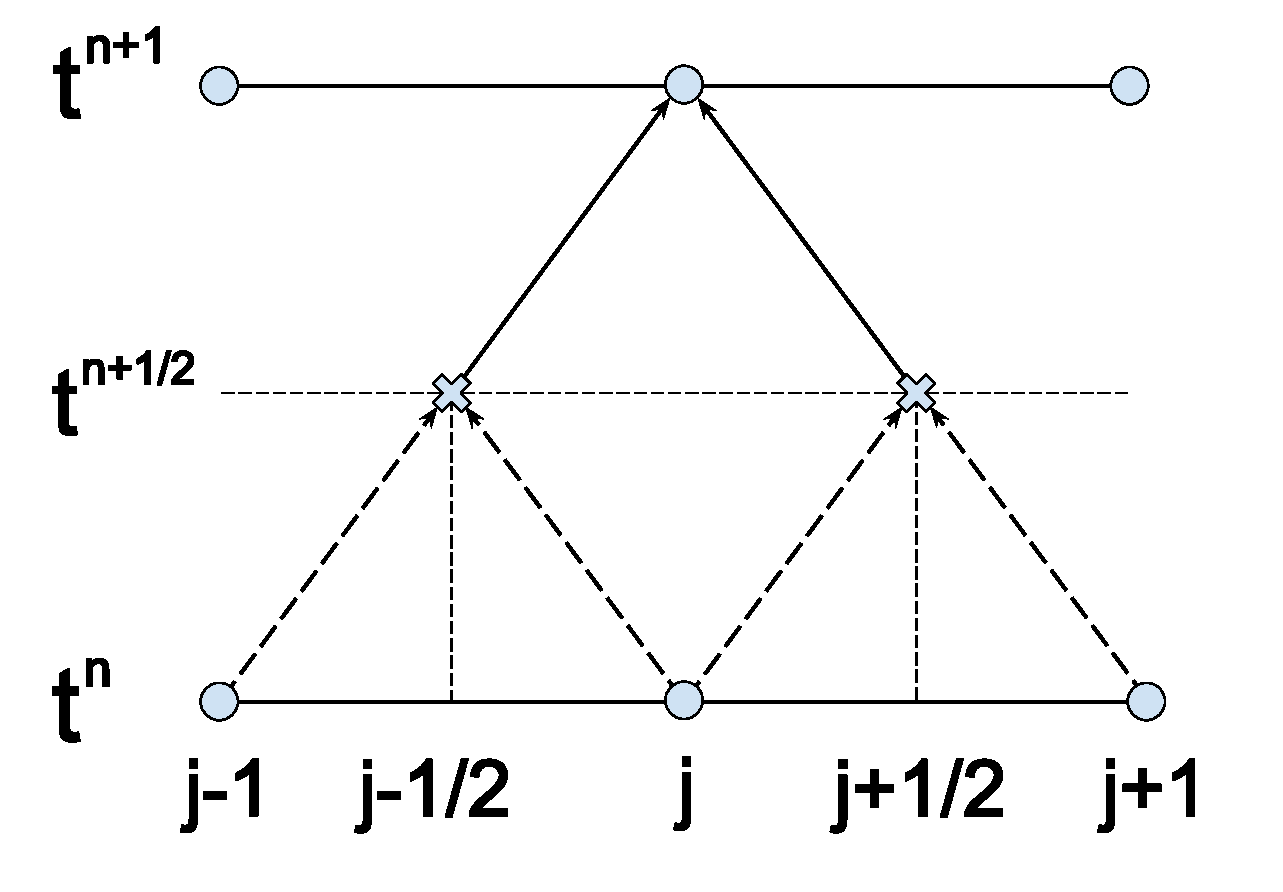
\includegraphics[width=0.8\textwidth]{Lax-Wendroff.pdf}
		\caption{Консервативный двухшаговый метод Лакса-Вендроффа на пространственно - временной сетке.}
		\label{LW_picture}
	\end{figure}
	Сетка для вычислений вводится следующим образом. Длина рассматриваемой области $l$ делится на выбранное количество ячеек $N$ в итоге получаем сетку с количеством ячеек $j$ - 
	\[
		0 \leqslant j \leqslant N .
	\]
	Ячейки с номерами 0 и N считаются граничными. Значения в этих ячейках определяются начальными условиями и остаются постоянными на протяжении всего расчёта, либо устанавилваются наперёд заданной функцией, зависящей от времени. То есть граничные условия задаются в виде:
	\begin{equation}\label{Dirihle}
		\mathbf{u}_0^n = \mathbf{u}_0^0	\:,	\qquad	\mathbf{u}_N^n = \mathbf{u}_N^0 \:,
	\end{equation}
	в случае граничных условий типа Дирихле. Если использовать граничные условия Неймана, то они будут иметь вид:
	\begin{equation}
		\diffp{\mathbf{u}_{0}}{t} = \diffp{\mathbf{u}_{N}}{t} = 0 .
	\end{equation}
	В этом случае нужно непосредственно аппроксимировать граничные условия методом конечных разностей. И непосредственно вычислять на каждом шаге по времени. 
	Для решения задачи о линейном переносе и о распаде разрыва ограничимся граничными условиями в виде \eqref{Dirihle}.
		
	\section{Задача о линейном переносе}\label{transfer}
	Рассмотрим одно из уравнений вида \eqref{dudt}, являющееся законом сохранения массы в дифференциальнй форме - уравнение переноса:
	\begin{equation}\label{eqTransfer}
		\diffp{\rho}{t} + \nabla ( \rho \mathbf{v} ) = 0 .
	\end{equation}
	В одномерном случае $\mathbf{u} = \rho$ и $\mathbf{F} = \rho v$. Разностная схема соответствует приведённым в разделе \ref{Lax-Wendroff} уравнениям \eqref{LW_helper} -- \eqref{LW_main}.
	
	Начальные условия:
	\begin{equation}\label{initTransfer}
		\begin{cases}
			\left.\mathbf{u}\right|_{t_0} = 0.8\:;		&		0.4 \leqslant x \leqslant 0.8 \, ,	\\
			\left.\mathbf{u}\right|_{t_0} = 0.4\:;		&		x < 0.4\,; x > 0.8 \, .
		\end{cases}
	\end{equation}
	\[
		\begin{aligned}
			x \in [0, 1] \\
			t \in [0, T]
		\end{aligned}
	\]
	При постоянном $v$ аналитическим решением уравнения адвекции является функция:
	\begin{equation}
		\mathbf{u}(t) = \mathbf{u_0}(x - vt) \: ,
	\end{equation}
	где $v = 1$ -- скорость распространения возмущения. 
	
	Таким образом, решением уравнения \eqref{eqTransfer} в момент времени $t = 0.3$ сек. будет начальный профиль \eqref{initTransfer}, сдвинутый вправо по оси x. 
	Ниже, на рисунке \ref{initTransferPlot} показано начальное распределение, которое, очевидно, полностью совпадает с заданными начальными условиями. 
	\begin{figure}[h]
		\centering
		\includegraphics[width=0.8\textwidth]{initial-transfer.pdf}
		\caption{Начальное распределение плотности. Линией показано точное значение, маркерами - соответствующий численный аналог для сетки с количеством ячеек 30, 100 и 1000.}
		\label{initTransferPlot}
	\end{figure}
	\begin{figure}[!h]
	\centering
	\includegraphics[height=0.8\textheight]{transfer.pdf}
	\caption{Решения уравнения переноса в момент времени $t = 0.3$ c. Слева показаны аналитическое и  численные решения. Справа показана относительная ошибка. Число Куранта равно 0.2, 0.6, 0.99 на рисунках сверху-вниз, соответственно.}
	\label{TransferPlot}
	\end{figure}
	На рисунке \ref{TransferPlot} показаны профили плотности через три десятых доли секунды от начала расчёта. При уменьшении значения числа Куранта отклонения от аналитического решения заметно увеличиваются, причем абсолютное значение погрешности остаётся примерно одинаковым, а размазывается профиль распределения вдоль оси x.
	Отклонения проявляются особенно сильно на резких перепадах, что связано с численной диффузией при использовании разностной схемы. 
	Также, рисунок \ref{TransferPlot} показывает, что схема согласованна. То есть, при увеличении числа ячеек численное решение стремится к аналитическому. 
	При числе Куранта $=0.99$ в ячейке, соответствующей разрыву относительная погрешность достигает $\approx 0.4$, однако в соседних ячейках погрешность уже на порядок ниже, а через несколько ячеек погрешность стремится к нулю. 
	Эффект, вызываемый численной диффузией возможно устранить только сильным усложнением схемы (четвертым порядком точности), либо введением специальной искусственной вязкости \cite{Richtmayer}, тогда фронт ударной волны уширится, и максимальное значение относительной погрешности будет меньше. 
	
	

%	\begin{figure}
%		\centering
%		\includegraphics[width=0.8\textwidth]{transfer-on-time.pdf}
%		\caption{Распределение плотности в момент времени $t = 0.3$ секунды. Точное решение показано синей линией. Численное решение показано треугольными маркерами для сетки с 10 000 ячеек, численное решение для сетки со 100 ячейками показано круглыми маркерами.}
%		\label{transferPlot}
%	\end{figure}
%	\begin{figure}
%		\centering
%		\includegraphics[width=0.8\textwidth]{transfer-mistake.pdf}
%		\caption{Относительная погрешность численного решения. Показано два случая (в зависимости от количества ячеек), по оси абсцисс выбран масштаб, где ошибка наиболее сильно проявляется.}
%		\label{transferMistake}
%	\end{figure}
	

	\section{Задача о гидродинамическом разрыве}\label{hydrodynamics}
	\subsection{Основные уравнения}
	%Potter p.272
	Уравнения идеальной гидродинамики в дифференциальной форме относительно неподвижной системы отсчёта:
	\begin{gather}\label{eqHydro}
		\diffp{\rho}{t} + \nabla ( \rho \mathbf{v} ) = 0 ,	\\[10pt]
		\diffp{\rho \mathbf{v}}{t} + (\nabla \rho \mathbf{v}) \mathbf{v} = -\nabla p ,	\\[10pt]
		\diffp{}{t}\left(\rho \varepsilon + \frac{1}{2} \rho v^2 \right) + 
						\nabla \left\{ \left( \frac{1}{2} \rho v^2 + \rho \varepsilon + p \right)\mathbf{v}\right\} = 0 ,
	\end{gather}
	где $\varepsilon$ -- удельная внутренняя энергия. Для иделального газа она выражается как:
	\begin{equation}
		\varepsilon = \dfrac{kT}{m(\gamma-1)} = \dfrac{p}{\rho (\gamma - 1)} ,
	\end{equation}
	где $\gamma$ -- показатель адиабаты (отношение теплоемкостей), $m$ -- масса молекулы (либо атома), $k$ -- постоянная Больцмана, $T$ - температура. 

	%Potter p.319
	Уравнения гидродинамики можно записать в консервативной форме следующим образом,	
	где векторы физических величин и потоков равны, соответственно:
	\begin{equation}
	\mathbf{u}	=	\begin{vmatrix}
						\rho								\\
						\rho v								\\
						\frac{1}{2}\rho v^2 + \rho \varepsilon		
					\end{vmatrix} , \qquad	
	\mathbf{F}	=	\begin{vmatrix}
						\rho v								\\
						\rho v^2 + p								\\
						\left(\rho \varepsilon + \frac{1}{2}\rho v^2 + p\right)v	
	\end{vmatrix}	.		
	\end{equation}
	
	Тогда разностная схема для решения уравнений идеальной гидродинамики двухшаговым методом Лакса-Вендроффа будет выглядеть следующим образом:
	
	\textit{Вспомогательный шаг:}
	\begin{gather}\label{HydroHelper}
	\rho_{j+1/2}^{n+1/2} = \frac{1}{2} \left(\rho_{j}^{n} + \rho{u}_{j+1}^{n}\right)
		- \frac{\Delta t}{2 \Delta x}	,	\\
	(\rho v)_{j+1/2}^{n+1/2} = \frac{1}{2} \left((\rho v)_{j}^{n} + (\rho v)_{j+1}^{n}\right)
	- \frac{\Delta t}{2 \Delta x}		,						
	\end{gather}
	\begin{multline}
		\left(\frac{\rho v^2}{2} + \rho \varepsilon	\right)_{j+1/2}^{n+1/2} = \\
		\frac{1}{2} \left(\left(\frac{\rho v^2}{2} + \rho \varepsilon	\right)_{j}^{n} 
		+ \left(\frac{\rho v^2}{2} + \rho \varepsilon	\right)_{j+1}^{n}\right) \\
		- \frac{\Delta t}{2 \Delta x}	.
	\end{multline}
	
	Для вычисления потоков примитивные переменные --- $v, \varepsilon$ выражаются из вектора консервативных переменных $\mathbf{u}$. Давление определяется с помощью полученных значений из уравнения состояния:
	
	\begin{equation}
		p = \rho \varepsilon (\gamma -1).
	\end{equation}
	
	Потоки и, соответственно, новые значения примитивных переменных вычисляются после каждого промежуточного и основного шага.
	
	\textit{Основной шаг:}
	\begin{gather}\label{HydroMain}
	\rho_{j}^{n+1} = \rho_{j}^{n} - \frac{\Delta t}{\Delta x} \left(
		(\rho v)_{j+1/2}^{n+1/2} - (\rho v)_{j-1/2}^{n+1/2}				 \right) , \\
	(\rho v)_{j}^{n+1} = (\rho v)_{j}^{n} - \frac{\Delta t}{\Delta x} \left(
		(\rho v^2 + p)_{j+1/2}^{n+1/2} - (\rho v^2 + p)_{j-1/2}^{n+1/2}				 \right) ,
	\end{gather}
	\begin{multline}
		\left(\frac{\rho v^2}{2} + \rho \varepsilon	\right)_{j}^{n+1} = 
		\left(\frac{\rho v^2}{2} + \rho \varepsilon	\right)_{j}^{n} -
		\\ - \frac{\Delta t}{\Delta x} \left[
		\left(\left\{\rho \varepsilon + \frac{1}{2}\rho v^2 + p\right\}v\right)_{j+1/2}^{n+1/2} - \right. 
		\\\left. - \left(\left\{\rho \varepsilon + \frac{1}{2}\rho v^2 + p\right\}v\right)_{j-1/2}^{n+1/2} \right] .
	\end{multline}
	
	\subsection{Начальные условия}
	Рассмотрим задачу о распаде произвольного разрыва со следующими начальными условиями:
	\begin{equation}
	\begin{cases}
		\left.\rho \right|_{t_0} = 1 \:;		&\quad		0 \leqslant x \leqslant 1 \, ,	\\
		\left. v   \right|_{t_0} = 0 \:;		&\quad		0 \leqslant x \leqslant 1 \, ,	\\
		\left. p   \right|_{t_0} = 3 \:;		&\quad		0 \leqslant x < 0.5 \, ,	\\
		\left. p   \right|_{t_0} = 1 \:;		&\quad		0.5 \leqslant x \leqslant 1 \, .	
	\end{cases}
	\end{equation}	
	
	Эти условия соответствуют перепаду давления (существующей перегородкой) на отметке $x = 0.5$. В момент времени $t = 0$ перегородку убирают и в расчётной области вправо (вдоль оси $x$) начинает распространяться ударная волна \cite{Zeldobich}. За ударной волной следуюет возмущенная область и контактный разрыв. Влево от начального положения $x = 0.5$ распространяется волна разрежения.
	
	\subsection{Результаты}
	Уравнения \eqref{eqHydro} решаются численно в соответствии со схемой \eqref{HydroHelper}, \eqref{HydroMain}. На рисунке \ref{ShockwavePlot} представлено полученное решение в момент времени $t = 137$мс. По профилю плотности хорошо различимы области распространения волн. Ударная волна находится на $x = 0.73$, контактный разрыв на $x = 0.57$, волна разрежения находится в диапазоне $ 1.9 \leqslant x \leqslant 0.3 $. В соответствии с теорией \cite{Rozhd} рисунок показывает что давление непрерывно на контактном разрыве, на ударной волне все величины испытывают скачок, и весь газ двигается в правую сторону (туда, где изначально давление было ниже). Эффекты численной диффузии порождают осцилляции на скачках физических величин. На рисунке \ref{ShockwavePlot2} представлены результаты расчёта с другими параметрами (число Куранта = 0.5, количество ячеек на расчётной сетке - 100). С этими параметрами более ярко выражены численные эффекты и так как количество ячеек меньше, то осцилляции даже не успевают затухать на всей площади области между ударной волной и контактным разрывом. Следовательно для сглаживания этих эффектов следует выбирать расчётную область с большим количеством ячеек, благо, современные вычислительные машины позволяют это делать.
	
	\begin{figure}%[!h]
		\centering
		\includegraphics[width=\textwidth]{sh_c9.pdf}
		\caption{Численное решение уравнений гидродинамики в задаче о распаде произвольного разрыва. Момент времени $t = 137$мc. Число Куранта в данном расчёте равно 0.9. Количество ячеек - 1000.}
		\label{ShockwavePlot}
	\end{figure}

	\begin{figure}%[!h]
		\centering
		\includegraphics[width=\textwidth]{sh_c5_N100.pdf}
		\caption{Численное решение уравнений гидродинамики в задаче о распаде произвольного разрыва. Момент времени $t = 0.14$cек. Число Куранта - 0.5, количество ячеек - 100.}
		\label{ShockwavePlot2}
	\end{figure}
	\newpage
	\section{Заключение}
	Во время прохождения практики были выполнены поставленные задачи. Изучен численный метод решения уравнений гиперболического типа - двухшаговый метод Лакса-Вендроффа. Написан код на языке С/С++ реализующий данный метод в виде консольной программы. Программа имеет возможность дополнения новыми блоками, для решения более сложных задач. Проведены тесты на задаче с хорошо известным аналитическим решением - задача о линейном переносе. Приведено аналитическое и численное решение уравнения адвекции с различными параметрами. Варьировалось количество ячеек на сетке и число Куранта. Показана сходимость метода, то есть при увеличении количества ячеек численное решение стремится к аналитическому. Далее, численно была решена задача о распаде произвольного разрыва. Полученные результаты согласуются с результатами других авторов \cite{Bisikalo}, что подтверждает корректность написания метода и позволяет использовать его для решения более комплексных задач.
	
	
%	\subsection{Аналитическое решение}
%	Задача о распаде произвольного разрыва - стандартная задача нахождения аналитического решения нестационарных уравнений механики сплошных сред. В случае, соответствующим заданным начальным условиям решения уже известны и опубликованы рядом авторов, например - (Зельдович, Ландау).
%	
%	В произвольный момент времени, решения для различных областей будут иметь вид (слева-направо):
%	
%	\textit{Невозмущенное вещество слева:}
%	\begin{equation}
%		x < 0.5 - c_L t		\qquad
%		\begin{cases}
%		v (x)		=	0		\\
%		\rho (x)	=	\rho_L	\\
%		p (x)		=	p_L		\\
%		\end{cases}
%	\end{equation}
%	
%	\textit{Волна разрежения:}
%	\begin{equation}
%	0.5 - c_L t	<	x	<	(v_2 - c_2)t		\quad
%	\begin{cases}
%	v (x)		=	v_2 \dfrac{x + c_L t}{(v_2 - c_2 + c_L)t}		\\
%	\rho (x)	=	\rho_L \left(1 - \dfrac{\gamma - 1}{2} \dfrac{v(x)}{c_L}\right)^{\frac{2}{\gamma -1}}	\\
%	p (x)		=	p_L \left(1 - \dfrac{\gamma - 1}{2} \dfrac{v(x)}{c_L}\right)^{\frac{2\gamma}{\gamma -1}}	\\
%	\end{cases}
%	\end{equation}
%	
%	\textit{Область между волной разрежения и контактным разрывом:}
%	\begin{equation}
%	(v_2 - c_2) t <	x < v_2 t		\qquad
%	\begin{cases}
%	v (x)		=	v_2		\\
%	\rho (x)	=	\rho_2	\\
%	p (x)		=	p_2		\\
%	\end{cases}
%	\end{equation}
%	
%	\textit{Область между контактным разрывом и ударной волной:}
%	\begin{equation}
%	v_2 t <	x < D t		\qquad
%	\begin{cases}
%	v (x)		=	v_2		\\
%	\rho (x)	=	\rho_1	\\
%	p (x)		=	p_2		\\
%	\end{cases}
%	\end{equation}
%	
%	\textit{Невозмущенное вещество справа:}
%	\begin{equation}
%	v_2 t <	x < D t		\qquad
%	\begin{cases}
%	v (x)		=	0		\\
%	\rho (x)	=	\rho_R	\\
%	p (x)		=	p_R		\\
%	\end{cases}
%	\end{equation}
%	
%	Здесь использованы следующим обозначения: $c_L = \sqrt{\gamma \dfrac{p_L}{\rho_L}}$ --- скорость звука в невозмущенной среде слева, $v_2, p_2, c_2 = \sqrt{\gamma \dfrac{p_2}{\rho_2}}$ --- параметры газа между фронтом ударной волны и контактным разрывом, $D$ --- скорость ударной волны.
%	Требуемые параметры определяются из следующей системы уравнений, отвечающей законам сохранения и условиям Гюгонио:
%	
%	\begin{gather}
%		\rho_1 = \rho_R \dfrac{D}{D-v_2}	,\\[5pt]
%		D = \dfrac{p_2 - p_R}{\rho_R v_2}	,\\[5pt]
%		\dfrac{p_L}{\rho_L^\gamma} = \dfrac{p_2}{\rho_2^\gamma}	,\\[5pt]
%		p_2 = p_R \dfrac{(\gamma + 1)\rho_1 - (\gamma-1)\rho_R}
%						{(\gamma + 1)\rho_R - (\gamma-1)\rho_1}	,\\[5pt]		
%		v_2 = \dfrac{2}{\gamma-1}\left(c_L-c_2\right) = \dfrac{2c_L}{\gamma-1} \left(1 - \left(\dfrac{\rho_2}{\rho_L}\right)^{\frac{\gamma-1}{2}}\right)	.
%	\end{gather}
\newpage	
\bibliographystyle{utf8gost705u}  			% стилевой файл для оформления по ГОСТу
\bibliography{literature}     					% файл библиографической базы 
\addcontentsline{toc}{section}{Список литературы}
	
	
\end{document}